%!TEX root = ../../../report.tex
\section{3D printing} % (fold)
\label{sec:3d_printing}
The parts modeled for the project and shown in section \ref{sub:computer_aided_design}, contain complex geometries that can only be achieved by 3D printing or complex machining.
Due to its availability and low price, Fused Filament Fabrication (FFF) technology has been used to implement the parts although other methods were considered.
The goals of this project requires the use of rapid and low-cost prototyping. 
Due to its intrinsic iterative design and the constrained timing, a technology that allows fast modifications in the design is required.

The additive manufacturing (AM) refers to the process of creating a geometry by adding material.
Besides FFF, others technologies as Stereolithography (SLA) or Digital Light Processing (DLP) that make use of the light to solidify a photo-sensible liquid, generally give better accuracy but at the expense of a higher price.
In this line, powder based AM like Selective laser melting (SLM) and Selective laser sintering (SLS), give also a higher detail although the post-processing and posterior mechanical properties tend to be lower.

Inside of the FFF, there are several materials from which a part can be printed of.
Stand out polymers like Polylactide (PLA) and Acrylonitrile butadiene styrene (ABS), materials easily printable that have good physical properties.
Its price can be considered inexpensive when comparing with the other AM technologies presented.
The easy access to this technology, mainly powered by its low-cost tag, has caused an increase of the popularity of this kind of 3D printing giving as a result a big community.
The outcome of this has been a wide variety of printable filaments with exotic properties: from non-flamable PLA to carbon fiber reinforced parts with metal-like mechanical properties.

For this project FFF using PLA has been used.
The reasons are feasibility and rapidness.
The availability of multiple 3D printers and filaments made the selection of this technology straightforward.
The 3D printer used is a M Prime One \cite{m_prime_one} with a 0.4 mm noozle.
PLA of two different colors was available, Blue and Black (the color may change the mechanical properties of the final printed part, due to different additives are used), from the provider BQ.
All the parts have been printed at 0.2 mm layer height making use of free software slicers as Cura \cite{cura} and Slic3r \cite{slic3r}.
The Figure \ref{fig:3d_printing_gcode} shows the gcode visualization of Simplify3D \cite{simplify3d} of the left foot.
\begin{figure}[htb]
  \centering
  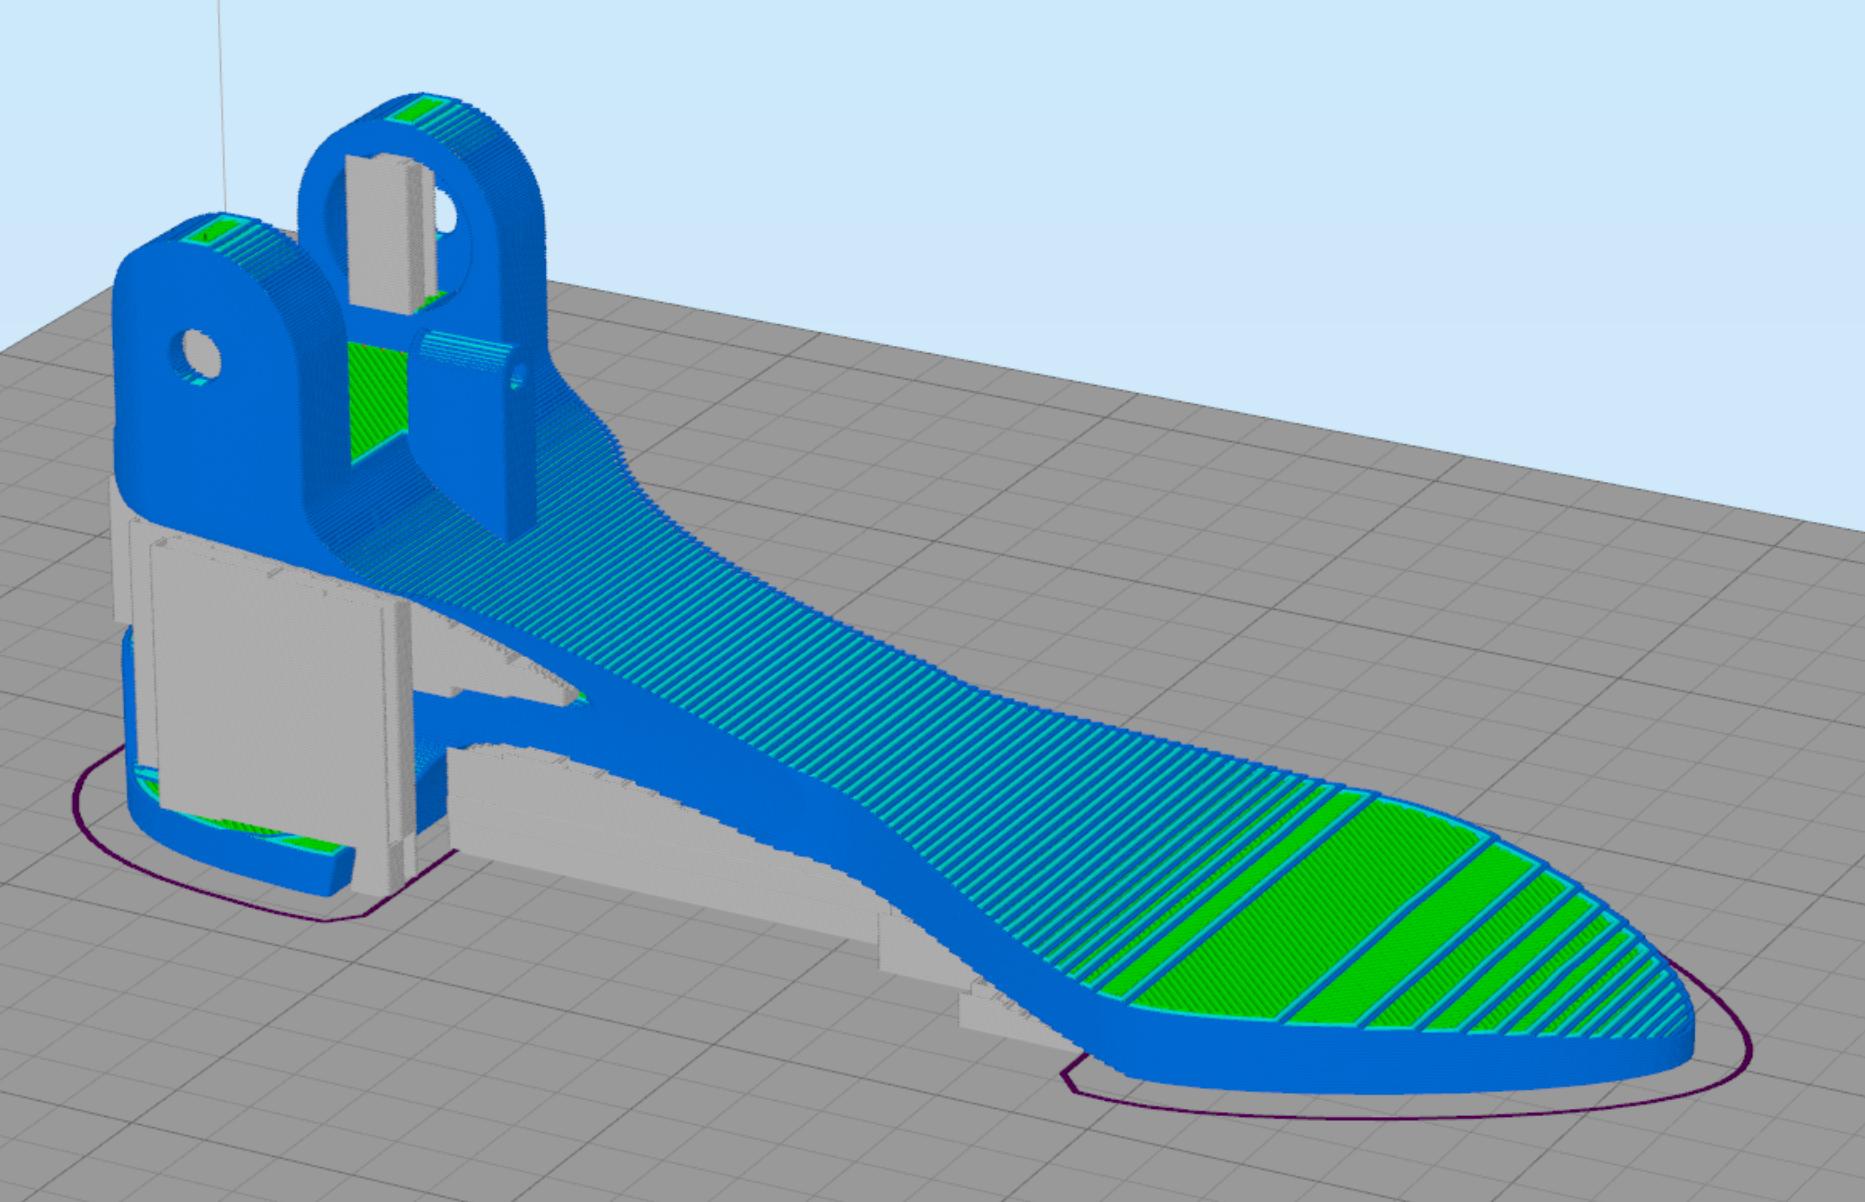
\includegraphics[width=0.75\textwidth]{figures/3d_printing_gcode}
  \caption{Gcode visualization from Simplify3D \cite{simplify3d}.}
  \label{fig:3d_printing_gcode}
\end{figure}
One of the intrinsic problems of this technology is the need of material support for some of the meshes.
Due to its stratification technique, if one of the higher layers lacked a lower one to be supported on, the material would fall causing problems in final part.
Nowadays, mostly all the slicers offer a material support solution that can vary but generally offering good results.
The Figure \ref{fig:photo_material_support} depicts two feet, one with material support and the other with it removed.

All the parts have been individually adjusted until the clearances have been as expected.
This has been achieved by an recursive process and a mix between experimental tests and other tools like the presented in \ref{sub:arc_compensation}.
In the Figure \ref{fig:photo_3d_printed} a detail of actual parts 3D printed and assembled in the robot are shown.

\begin{figure}[ht]
    \centering
    \begin{subfigure}[b]{0.49\textwidth}
        \includegraphics[width=\textwidth]{figures/photo_material_support.jpg}
        \caption{Feet with and without material support.}
        \label{fig:photo_material_support}
    \end{subfigure}
    \begin{subfigure}[b]{0.49\textwidth}
        \includegraphics[width=\textwidth]{figures/photo_3d_printed.jpg}
        \caption{Detail of 3D printed parts assembled.}
        \label{fig:photo_3d_printed}
    \end{subfigure}
    \caption{Photos of 3D printed parts.}
\end{figure}

  \subsection{Arc compensation in FFF} % (fold)
  \label{sub:arc_compensation}
  For the CAD models of the 3D printed parts, the clearances of the internal holes have been adjusted following \cite{arc_compensation}.
  The undersizing of internal holes is a common problem in this sort of technology due to the lack of information of the common-used exporting format: the STL.
  This only contains the 3D model expressed as a set of external triangles and its normal, which difficulties the correction of malformations inherent to this technology.

  In the case of the Fused Filament Fabrication (FFF), the material is extruded equally in both sides of the arc, as shown in \ref{fig:arc_compensation}. 
  However, in the side of the smaller curve, less material is needed.
  This correction can be calculated with the equation \ref{eq:r_arc_compensation}   being $t$ the noozle diameter, $R$ the desired internal hole radius and $r$ the corrected radius.
  \begin{equation}
    \label{eq:r_arc_compensation}
    r=\frac{t+\sqrt{t^2+4R^2}}{2}
  \end{equation}
  As an example, Klee suggests an internal hole of 4.4 mm in the case of the selected nuts \cite{klee}. 
  Thus, the diameter in the CAD model has been adjusted for this data and a noozle of 0.4 mm. The result is then show in \ref{eq:diameter_example}.

  \begin{equation}
    \label{eq:diameter_example}
    d=2r=\frac{t+\sqrt{t^2+4R^2}}{2}=0.4+\sqrt{0.4^2+4*2.2^2}=4.81
  \end{equation}

  \begin{figure}[tb]
    \centering
    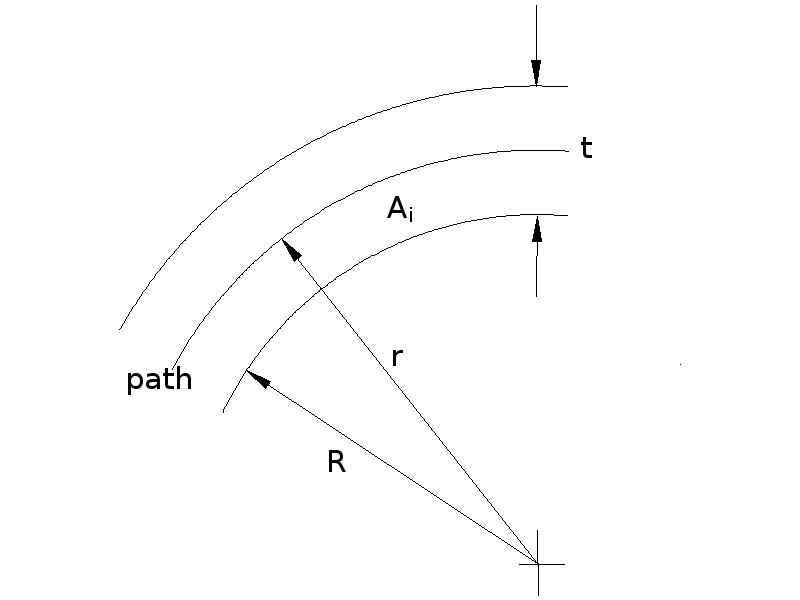
\includegraphics[width=0.5\textwidth]{figures/Arc-compensation}
    \caption{Technical representation of the generated arc when using FFF technology.}
    \label{fig:arc_compensation}
  \end{figure}
  % subsection arc_compensation (end)

% section 3d_printing (end)
